\documentclass[justified]{tufte-handout}
\usepackage{../braph2_tut}
%\geometry{showframe} % display margins for debugging page layout

\title{Group of Subjects with Functional Multiplex Data}

\begin{document}

\maketitle

\begin{abstract}
\noindent
For \emph{functional multiplex data}, you will upload a folder containing the functional files for different subjects, and different layers, that belong to the same group. For example, the functional multiplex values could correspond to brain activation signals derived from functional MRI data at different frequencies or time windows.  Later, a connectivity matrix will be computed for each layer using correlations in functional values between each pair of brain regions. This tutorial explains how to prepare and work with this kind of data.
\end{abstract}

%! FIG1 !%

\tableofcontents

\fig{figure}
	{fig:01}
	{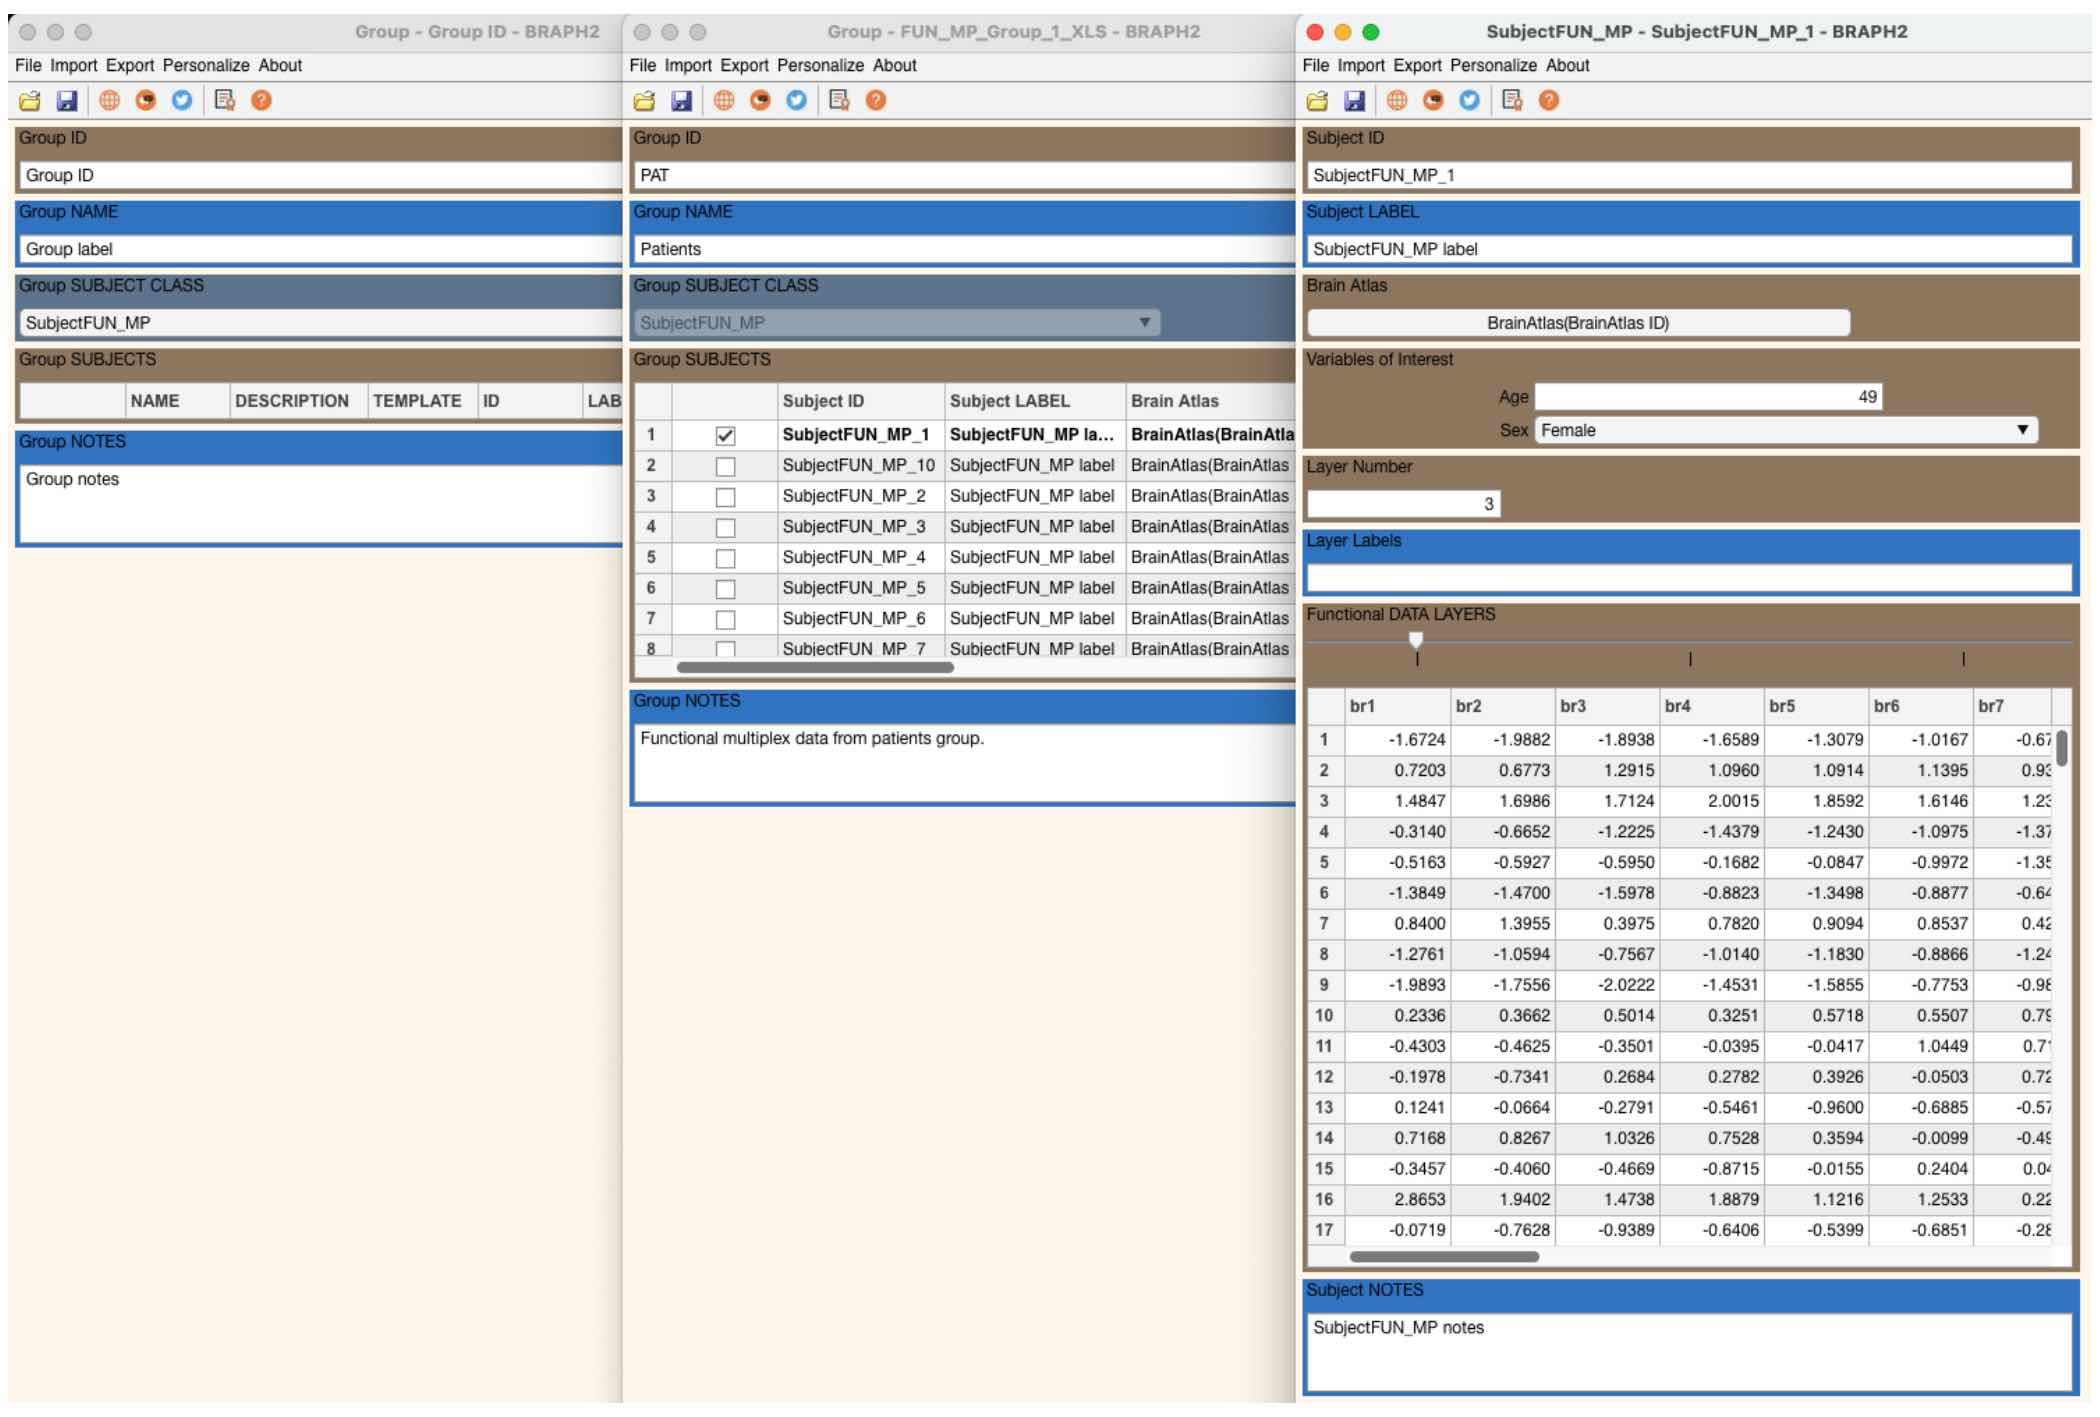
\includegraphics{fig01.jpg}}
	{GUI for a group of subjects with functional multiplex data}
	{
	Full graphical user interface to upload a group with functional multiplex data in BRAPH~2. 
	}

\clearpage
\section{Generation of Example Data}

If you do not have the \fn{Example data FUN\_MP XLS} folder inside \fn{functional multiplex}, then you can generate it by running the commands in \Coderef{cd:exampledata}.

\begin{lstlisting}[
	label=cd:exampledata,
	caption={
		{\bf Code to generate the example data folder.}
		This code can be used in the MatLab command line to generate the \fn{Example data FUN$\_$MP XLS} folder to the \fn{functional multiplex} pipeline folder.
	}
]
create_data_FUN_MP_XLS() ¥\circled{1}\circlednote{1}{generates the example functional multiplex XLS data folder.}¥
create_data_FUN_MP_TXT()  ¥\circled{2}\circlednote{2}{generates the example functional multiplex TXT data folder.}¥
\end{lstlisting}

\section{Open the GUI}

In most analyses, the group GUI is the second step after you have selected a brain atlas. You can open it by typing \code{braph2} in MatLab's terminal, which allows you to select a pipeline containing the steps required to perform your analysis and upload a brain atlas. After these steps have been completed you can upload your group's data directly (\Figref{fig:02}c-f) after clicking ``Load Group''. 

\fig{figure}
	{fig:02}
	{
	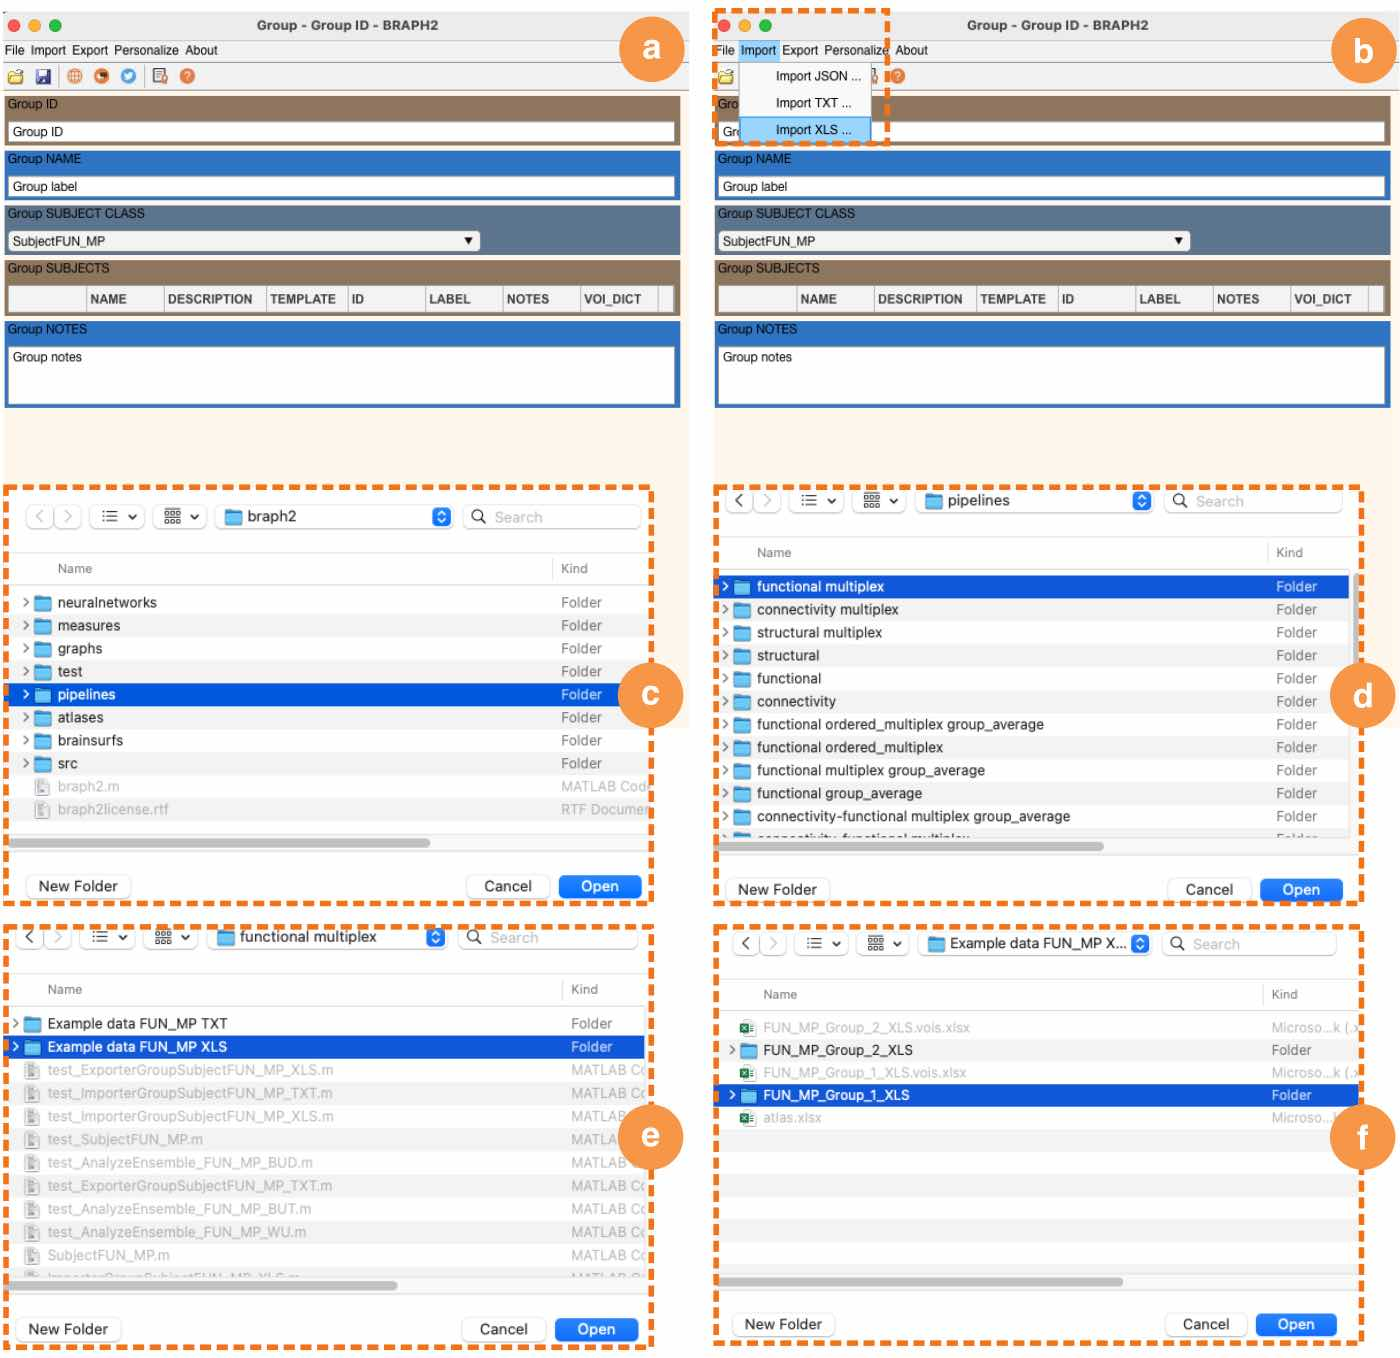
\includegraphics{fig02.jpg}
	}
	{Upload the data of a group of subjects}
	{
	Steps to upload a group of subjects with functional multiplex data using the GUI and an example dataset: 
	{\bf a} Open the group GUI.
	{\bf b} Import the folder with the functional multiplex files in XLS or TXT format (see below for details on their format).
	To upload the test functional multiplex data:
	{\bf c}-{\bf f} navigate to the BRAPH~2 folder \fn{pipelines}, {\bf d} \fn{functional multiplex},  {\bf e} \fn{Example data FUN\_MP XLS}, and {\bf f} select the folder with functional multiplex values of one group \fn{FUN\_MP\_Group\_1\_XLS}.
	}

%! FIG2 !%

\begin{tcolorbox}[
	title=GUI launch from command line
]
You can also open the GUI and upload the brain functional multiplex data using the command line (i.e., without opening an analysis pipeline) by typing the commands in \Coderef{cd:launch}. In this case, you can upload the data as shown in \Figref{fig:02}a-f.

\begin{lstlisting}[
	label=cd:launch,
	caption={
		{\bf Code to launch the GUI to upload a group of subjects with functional multiplex data.}
		This code can be used in the MatLab command line to launch the GUI to upload a group of subjects with functional multiplex data without having to open a pipeline.
	}
]
gr = Group('SUB_CLASS', 'SubjectFUN_MP');

gui = GUIElement('PE', gr);
gui.get('DRAW')
gui.get('SHOW')
\end{lstlisting}
\end{tcolorbox}

\section{Visualize the Group Data}

After completing the steps described in \Figref{fig:02}, you can see the data (\Figref{fig:03}a), and change the Group ID, name, and notes (\Figref{fig:03}b). 

\fig{figure}
	{fig:03}
	{
	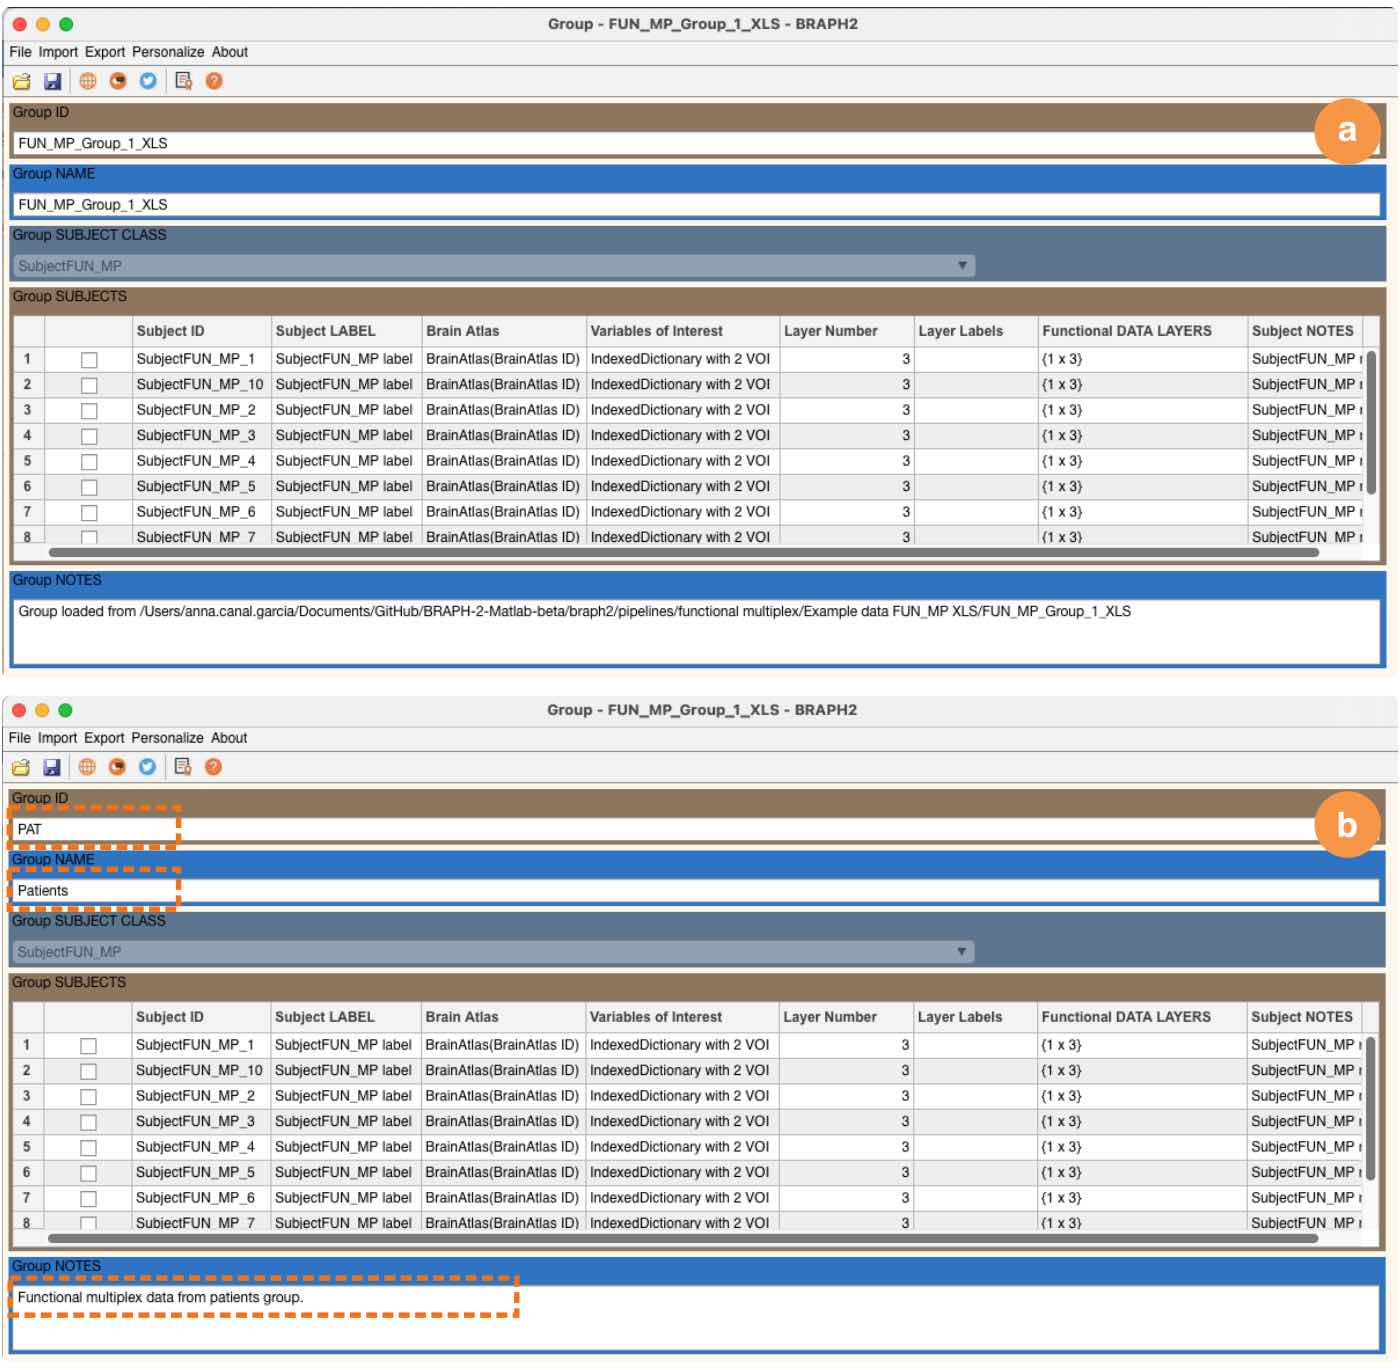
\includegraphics{fig03.jpg}
	}
	{Edit the group metadata}
	{ 
	{\bf a} The GUI of the group's functional multiplex data. 
	{\bf b} The information you see on this GUI that can be changed. In this example, we have edited the ID, name, and notes of the group but can also change the subject's specific information.
	}

%! FIG3 !%

\section{Visualize Each Subject's Data}

Finally, you can open each subject's functional multiplex values by selecting the subject, right click, and select ``Open selection'' (\Figref{fig:04}a), which shows the functional values from layer 1 (\Figref{fig:04}b). Here, you can also change the subject's metadata (ID, label, notes), its variables of interest, and the functional multiplex values.

\fig{figure}
	{fig:04}
	{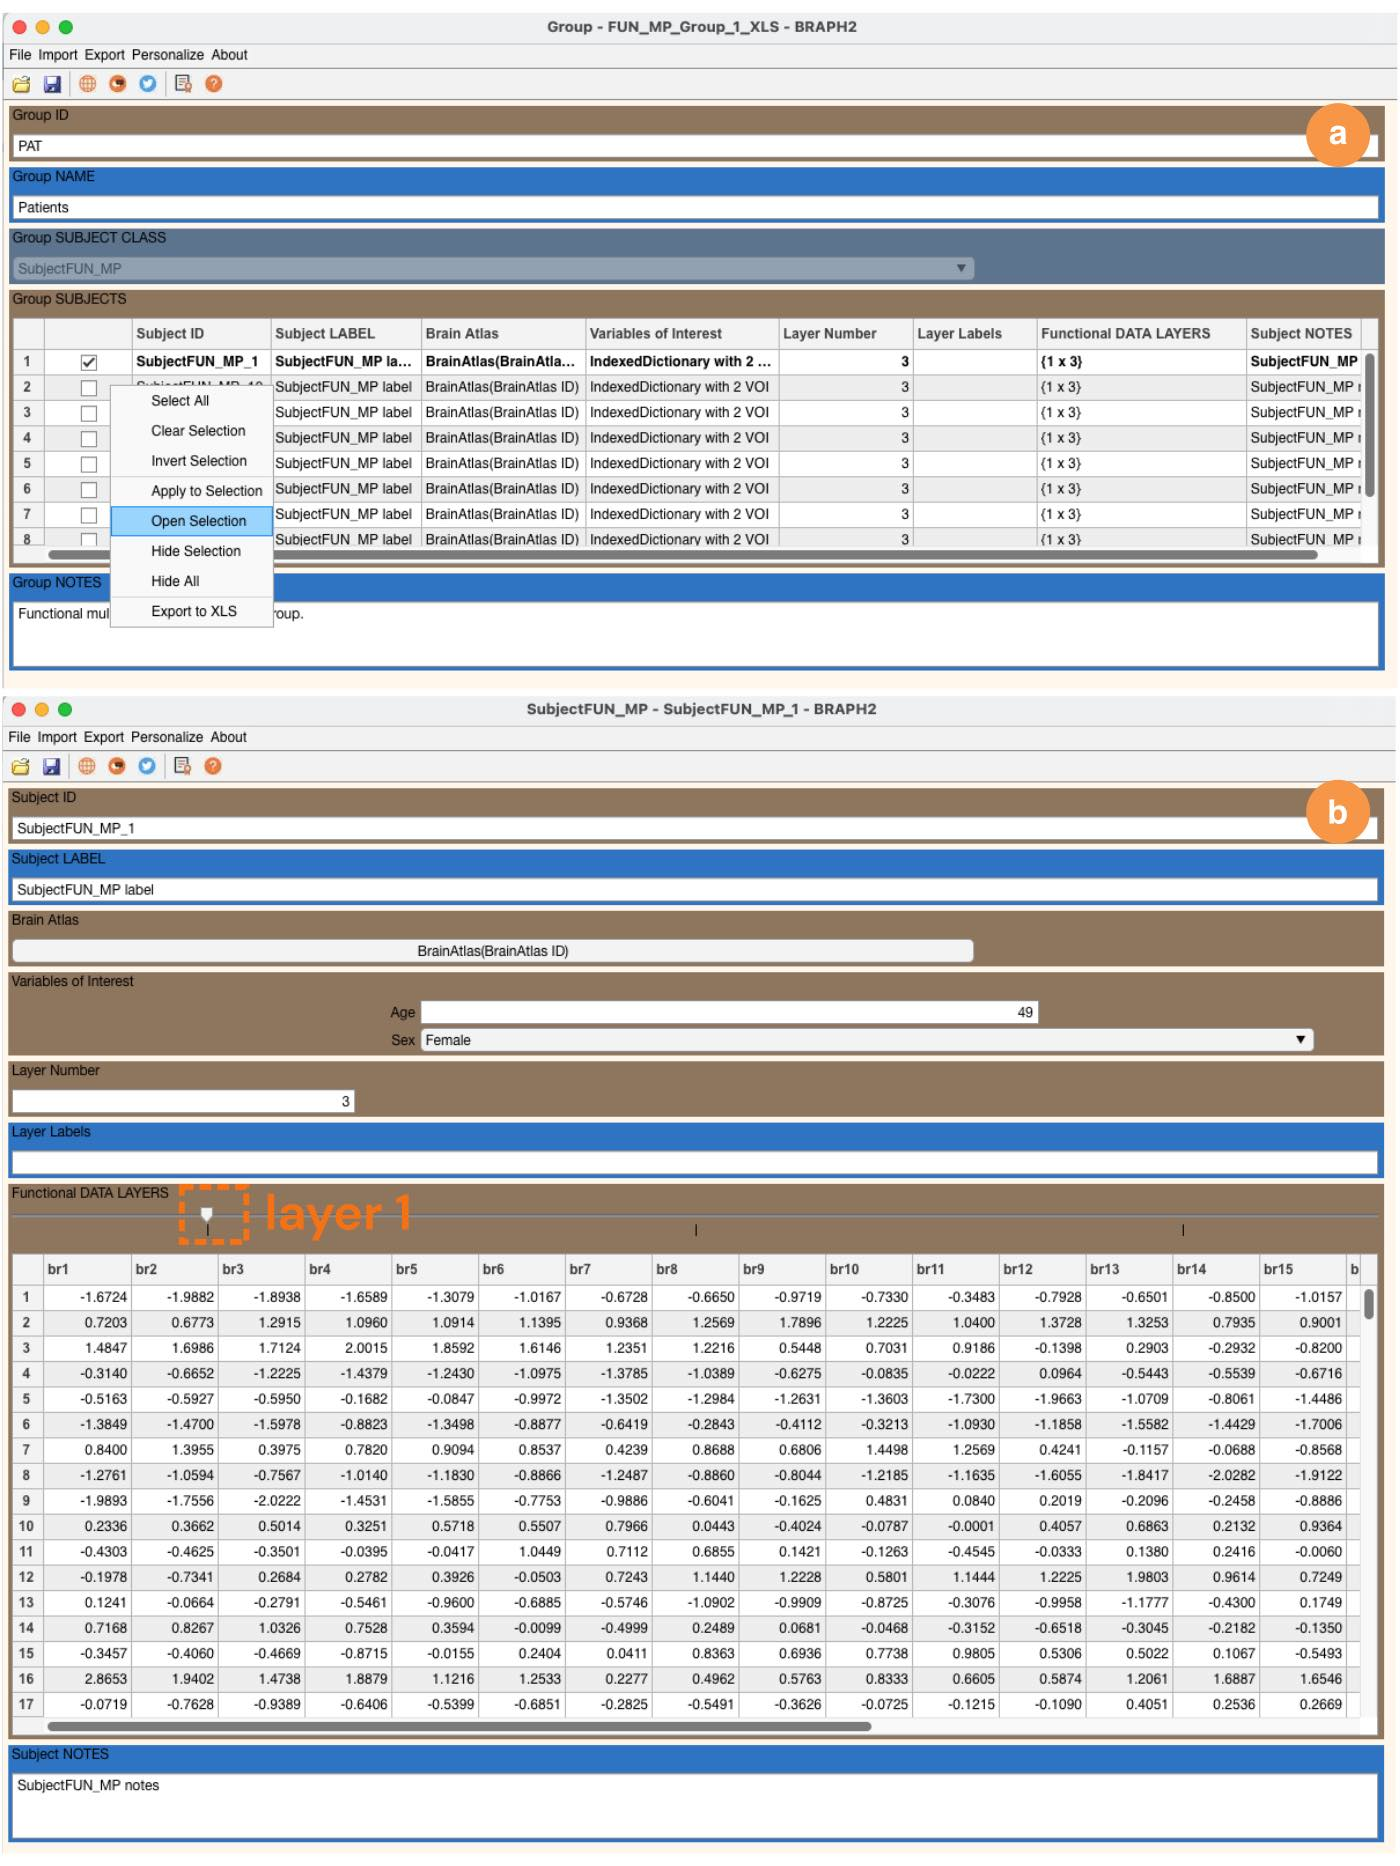
\includegraphics{fig04.jpg}
	}
	{Edit the individual subject data}
	{
	{\bf a}  Each subject's functional multiplex values can be opened by selecting the subject, right click, and select ``Open selection''
	{\bf b} In this subject GUI, it is possible to view and edit the metadata of the subject (ID, label, notes), its variables of interest (in this case, age and sex), and the functional multiplex values. 
	}

%! FIG4 !%

\clearpage
\section{Preparation of the Data to Be Imported}

To be able to import functional multiplex data into BRAPH~2, you need to include the functional values of each layer for all subjects in a single file in excel or text format. All functional layers' files should be inside one group folder. Below you can see how this file should look like.

\fig{figure*}
	{fig:05}
	{
	[h!]
	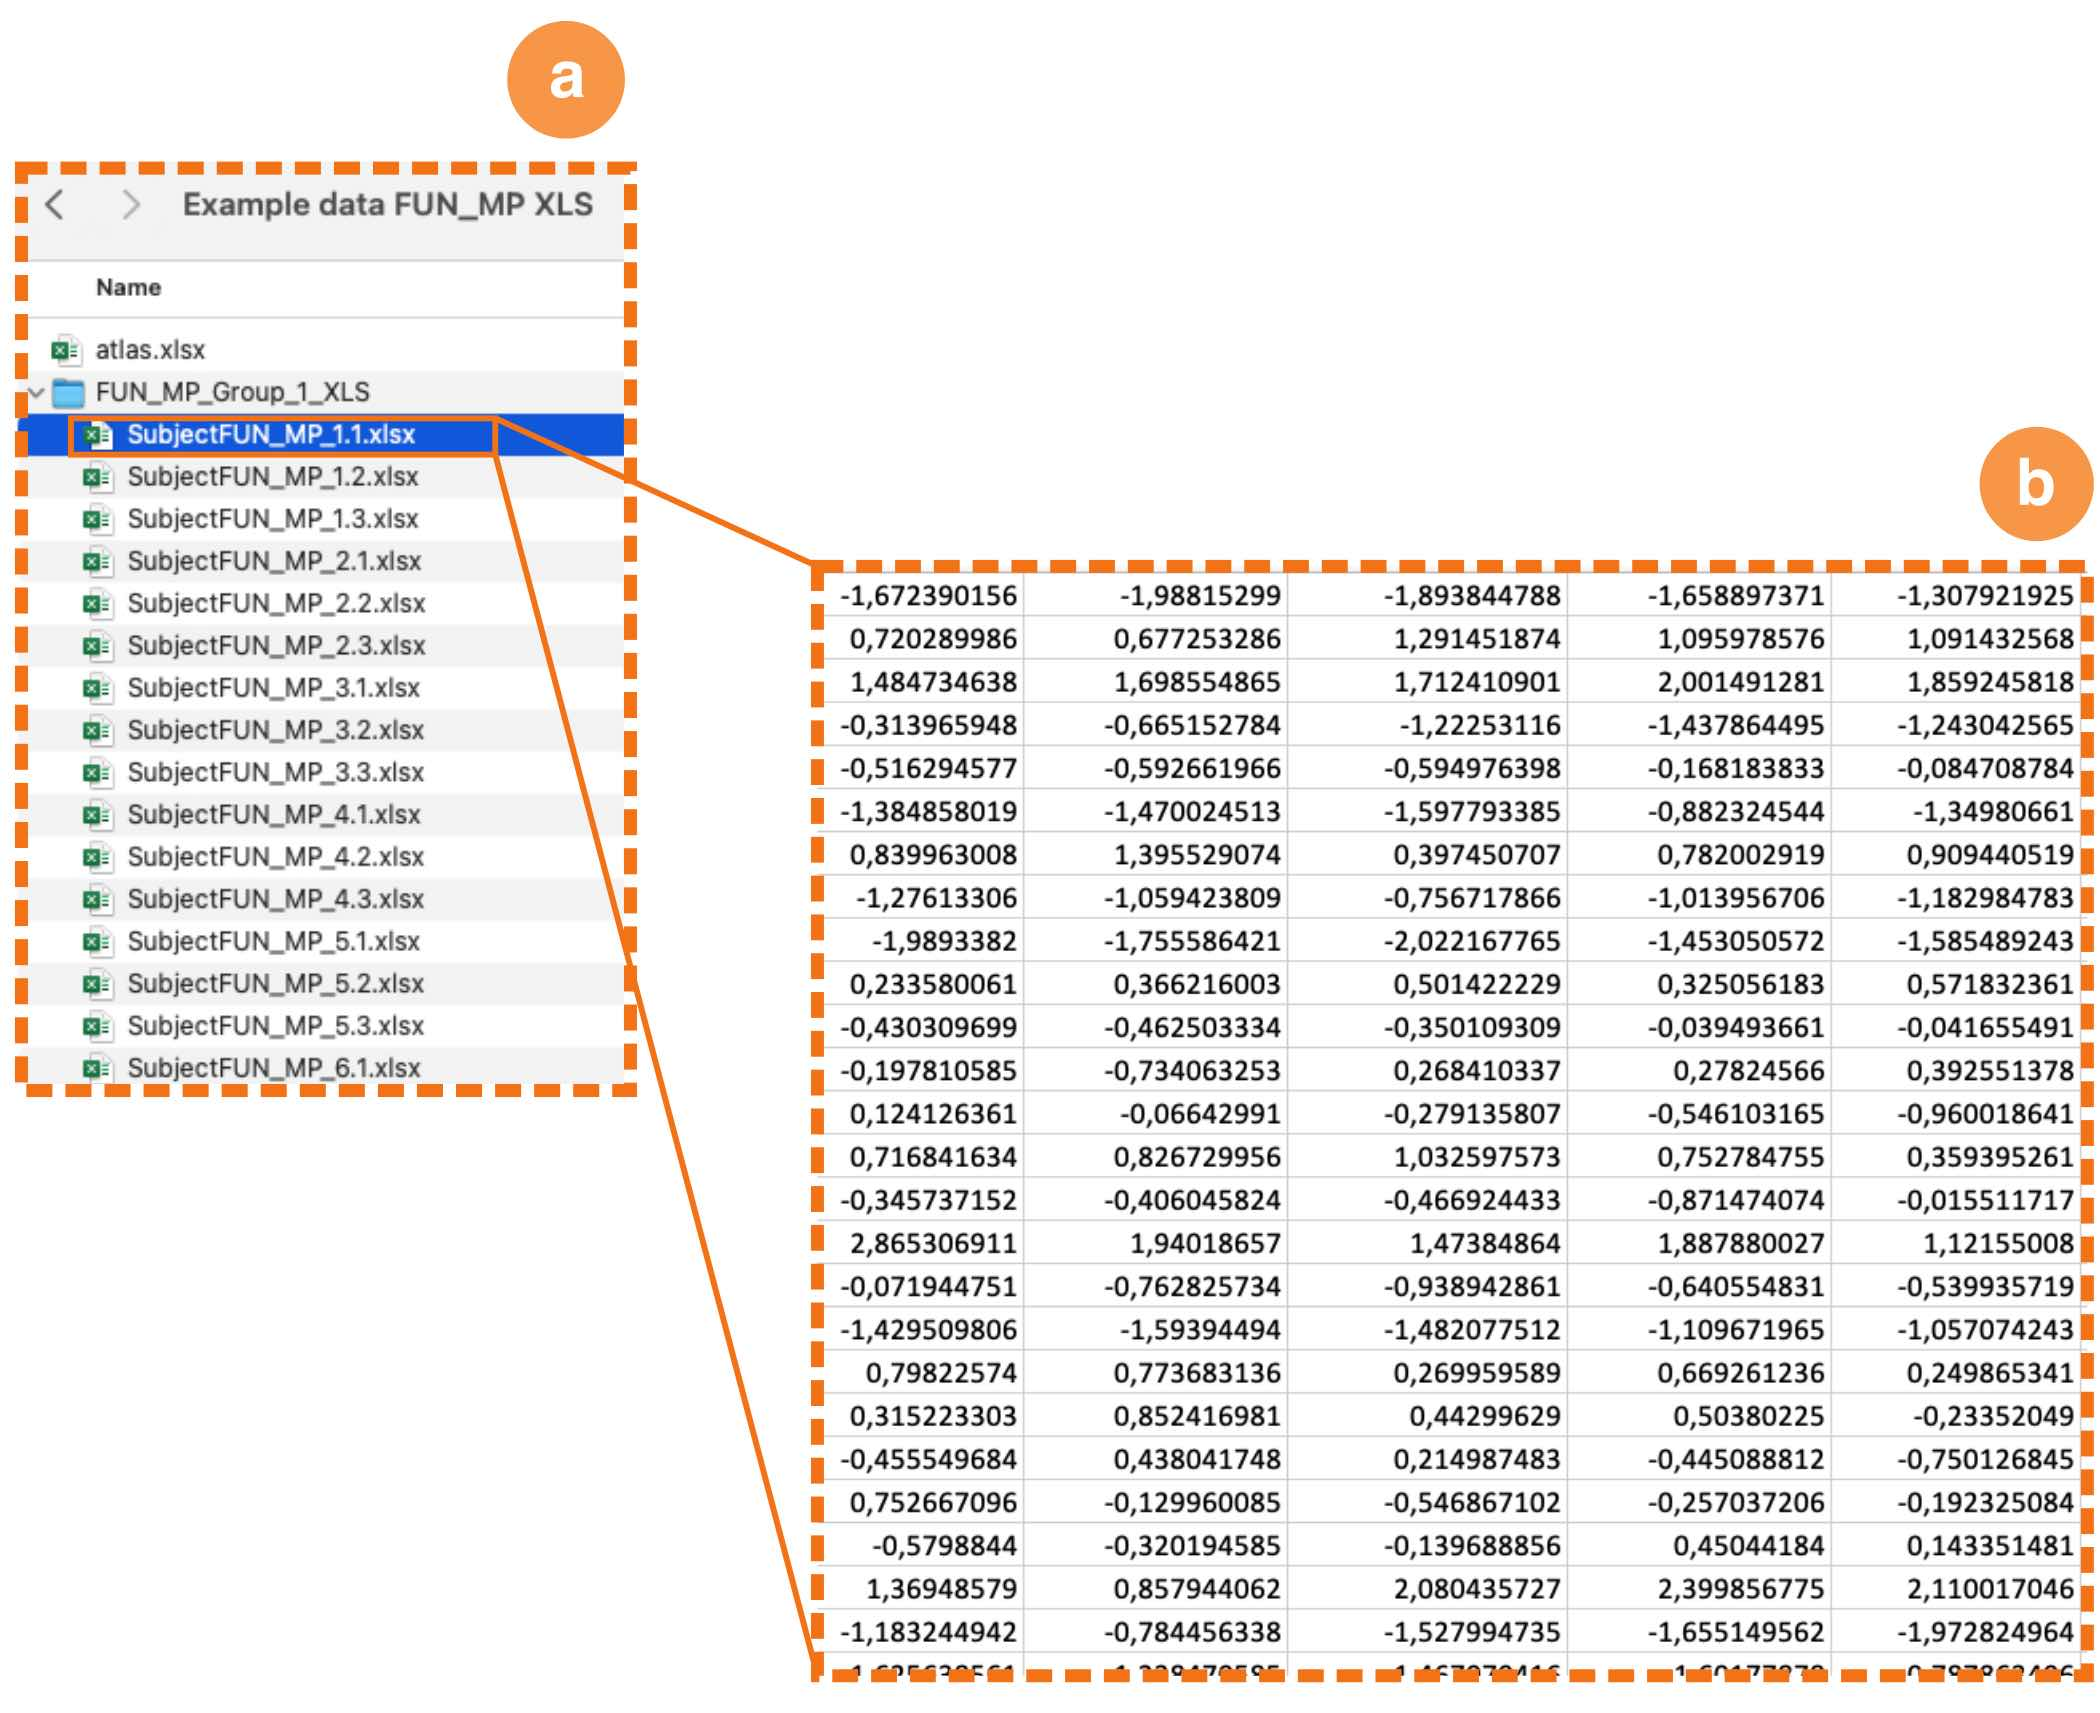
\includegraphics{fig05.jpg}
	}
	{Data preparation}
	{
	The data should be organised in the following format:
	{\bf a} The functional values of one layer from each subject belonging to the same group should be included in a single file (for example, \fn{FUN\_MP\_Group\_1\_xlsx}). 
	{\bf b} This file should contain the subject's IDs, label and any relevant notes, followed by the functional values for each brain region belonging to a brain atlas. In this example, the (simulated) values correspond to brain activation signals of 90 brain regions derived from functional MRI.
	}

%! FIG5 !%

\section{Adding Covariates}

\fig{figure*}
	{fig:06}
	{
	[h!]
	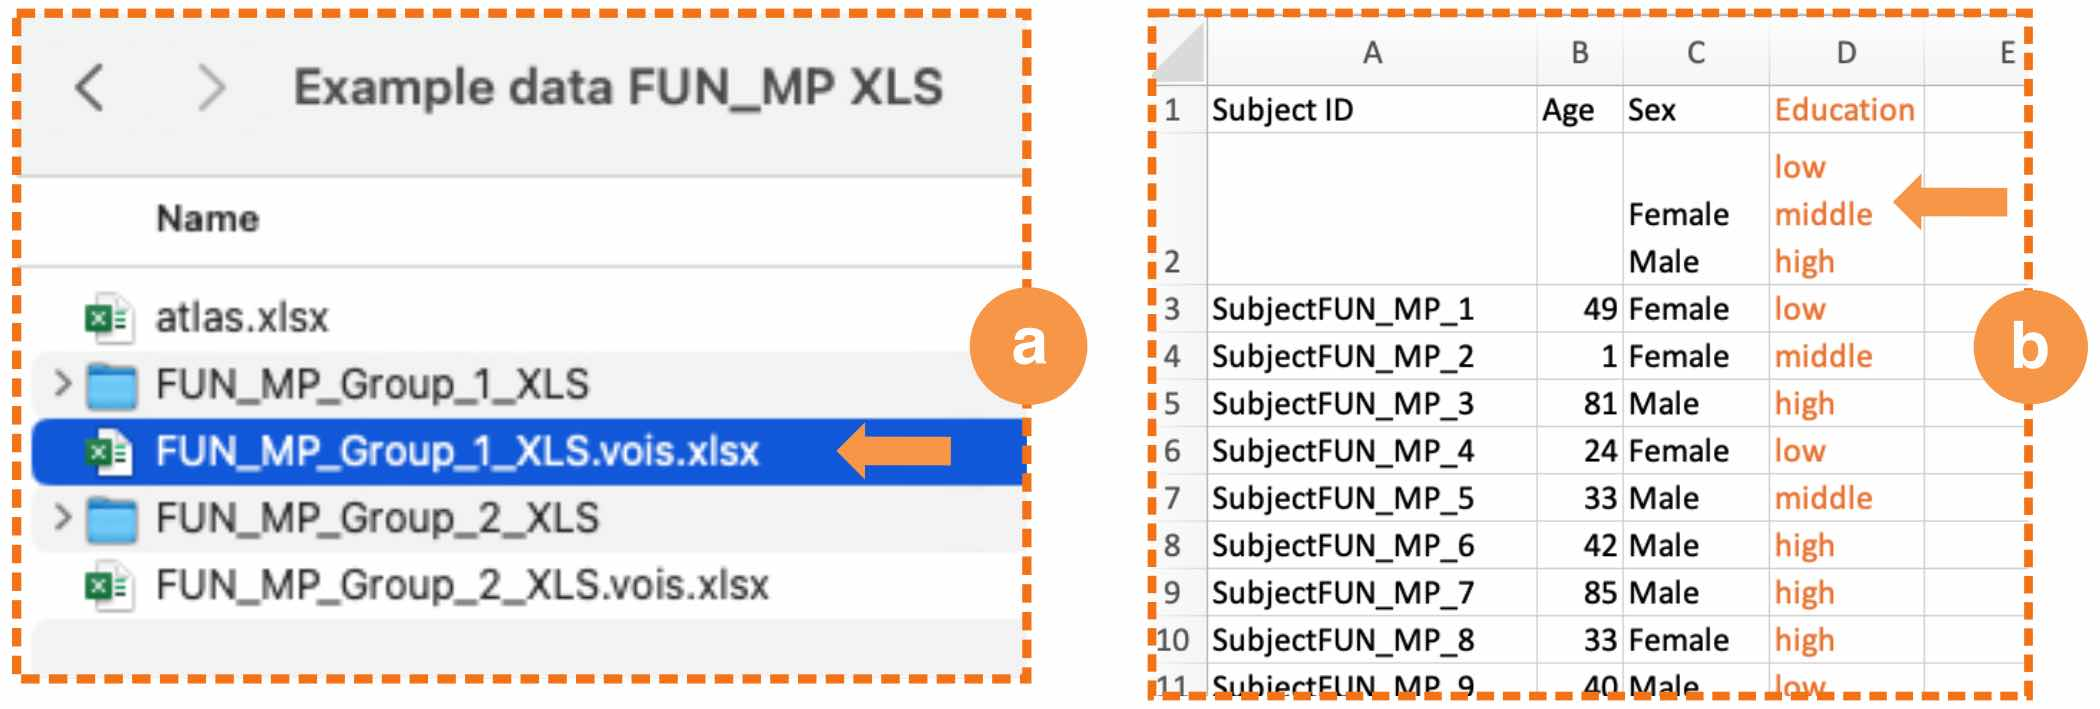
\includegraphics{fig06.jpg}
	}
	{Edit the Covariates}
	{
	Information that can be changed in the Covariates file: 
	{\bf a} The values of the variables of interest (vois).
	{\bf b} In case the vois are categorical, you can state which categories they have.
	}
	
It is very common to have \emph{variables of interest} (i.e., \emph{covariates} and \emph{correlates}) in an analysis. In BRAPH~2, 
these variables of interest should be included in a separate excel file placed just outside the group's folder and with the same name as the folder followed by \fn{.vois} (\Figref{fig:06}a). This file should have a specific format (\Figref{fig:06}b):
\begin{itemize}

\item {\bf Subject IDs (column A).}
Column A should contain the subject IDs starting from row 3.

\item {\bf Variables of interest (column B and subsequent columns).}
Column B (and subsequent columns) should contain the variables of interest (one per column). 
In this example we have ``Age'' and ``Sex'', as in the example file, as well as the additional ``Education''.
In each column, row 1 should contain the name of the variable of interest, row 2 should contain the categories separated by a return (only for categorical variables of interest, like ``Sex'' and ``Education''), and the subsequent rows the values of the variable of interest for each subject.

\end{itemize}	

%! FIG6 !%

\end{document}